Prime numbers are fundamental in the study of number theory; they are the `atoms' from which all other integers are built. Indeed, any whole number can be uniquely represented (up to multiplication by $\pm 1$ and re-ordering) as a product of prime numbers. This is known as the \textit{fundamental theorem of arithmetic}. The primes have fascinated mathematicians for hundreds of years, mainly due to their highly non-trivial nature. To quote Euler \cite{simmons_2019}: 
\begin{Quote}
\label{EulerQuote}
    \textit{``Mathematicians have tried in vain to this day to discover some order in the sequence of prime numbers, and we have reason to believe that it is a mystery into which the human mind will never penetrate."}
\end{Quote}
In addition to the beauty and mystery of the primes, they have very practical uses in cryptography such as the RSA algorithm \cite{Riesel1994}. Our aim therefore is to prove the great Euler wrong (to some extent!). The first natural question about the primes is simply `how many are there?'. This was known by Euclid over 2000 years ago \cite{ore_2012}.
\begin{proposition}
(Euclid, 300 BC) There are infinitely many prime numbers.
\end{proposition}
\begin{proof}
Euclid's classic proof is by contradiction and is particularly elegant. Assume there are finitely many primes, and enumerate them as $p_1, p_2, \dots, p_n$ in an exhaustive list. Then, set
\begin{equation}
    N = p_1 p_2 \dots p_n + 1. \nonumber
\end{equation}
None of the primes $p_i$ divide $N$, but either $N$ is prime or it has a prime dividing it. Consequently, there exists another prime not in the list $p_1, \dots p_n$, which is a contradiction.
\end{proof}
Broadly speaking, problems about the primes can be categorised as either \textit{global problems} or \textit{local problems}. The former are concerned with questions such as `how many', while the latter studies properties of individual primes $p_n$, such as the size of $p_{n+1} - p_n$. There is a wealth of unsolved problems in both categories, but the main focus of this report is to solve those of the global kind with analytic methods. According to Davenport \cite[p.~1]{davenport}, the adoption of such methods to tackle problems about primes arguably began with Dirichlet, whose 1837 memoir studied the existence of primes in arithmetic progressions. Such progressions are of the form 
\begin{equation}
    a, \quad a + q, \quad a + 2q, \quad a + 3q, \quad \dots \nonumber
\end{equation}
where $a$ and $q$ are integers. Note that if $a$ and $q$ share a common factor, then all numbers in the progression (with the possible exception of $a$) are not prime. It is therefore only interesting to study those progressions when $a$ and $q$ are coprime. It was conjectured long before the work of Dirichlet that such a progression always contains infinitely many primes - Dirichlet gave a proof of this with the (rather large) assumption of his \textit{class number formula} \cite[p.~1]{davenport}, the details of which we will not delve into. For certain examples, it is elementary to show that there are infinitely many primes. For example, consider the progression $4n + 3$, for non-negative integers $n$. Suppose there were finitely many primes of this form, say $p_1, \dots, p_n$, and consider the number 
\begin{equation}
    N = 4 p_1 \dots p_n + 3. \nonumber
\end{equation}
$N$ can be written as a product of primes, and since $N$ is odd these are either of the form $4n + 1$ or $4n + 3$. Moreover, none of these can be of the form $4n + 3$, as $N$ is not divisible by any of the $p_i$. Thus, $N$ is the product of primes of the form $4n + 1$, and we can easily check that this implies $N$ is also of the form $4n + 1$ - a contradiction. This method is limited: what if $q$ is not a number such as $4$, but is $400$, or $4000$? One of our first aims is to prove the existence of infinitely many primes in arithmetic progressions for \textit{arbitrary} coprime integers $q$ and $a$. This is known as Dirichlet's theorem.\\

Further advances in analytic number theory followed Riemann's memoir of 1859, which led to important results regarding the number of primes less than a given value. To this end, one studies the function $\pi(x)$, defined as the number of primes $p \leq x$. Gauss had conjectured early in his life that 
\begin{equation}
    \pi(x) \sim \frac{x}{\log x}, \ \textrm{as} \ x \rightarrow \infty \nonumber
\end{equation}
where $f(x) \sim g(x)$ if the limit of $f/g$ approches 1. He later refined his estimate to
\begin{equation}
    \pi(x) \sim \textrm{Li}(x) = \int_{2}^{\infty}\frac{\mathrm{d}t}{\log t}, \nonumber
\end{equation}
which actually gives a much sharper approximation (and implies his previous estimate by integration by parts). We note the numerical evidence detailed in Table~\ref{tab:my_label}.
\begin{table}[H]
    \centering
    \begin{tabular}{c|c|c|c}
        $x$ &  $\pi(x)$ & $\abs{\pi(x) - x/\log x}$ & $\abs{\pi(x) - \textrm{Li}(x)}$ \\
         \hline
        $10^{2}$ & $25$ & $3$ & $5$\\
        $10^{4}$ & $1229$& $143$ & $17$\\
        $10^{6}$ & $78498$& $6116$ & $130$\\
        $10^{8}$ & $5761455$& $332774$ & $754$\\
        $10^{10}$ & $455052511$ & $20758029$ & $3104$ \\
        % $10^{12}$ & $37607912018$ & $1416705193$ & $38263$\\
    \end{tabular}
    \caption[Errors in Gauss's approximations for $\pi(x)$.] {Errors in Gauss's approximations for $\pi(x)$. \protect\footnotemark}
    \label{tab:my_label}
\end{table}
\footnotetext{The On-Line Encyclopedia of Integer Sequences, published electronically at \url{https://oeis.org}. Sequences A006880, A057835, A057752. [Accessed: 26-04-2020]}
Note that the number of digits in the right-most column is always roughly half the number of digits in the left-most, suggesting the error in approximating $\pi(x)$ by $\textrm{Li}(x)$ is approximately $\sqrt{x}$. The problem of quantifying this error term, and proving that $\pi(x) \sim \textrm{Li}(x)$ is a central problem in this report. Gauss's conjecture was first proved independently by Hadamard and de la Vallée Poussin in 1896, extending the crucial work in Riemann's memoir, with a result known as the \textit{prime number theorem} \cite[p.~2]{heath-brown_2005}. \\


Results relating to $\pi(x)$ may then be extended using similar methods to results about $\pi(x; q, a)$, defined as the number of primes less than or equal to $x$ in the arithmetic progression $q n + a$. This is the ultimate aim of the report: to say something concrete about how the primes are distributed among each arithmetic progression with respect to a given $q$, and how many primes there are in each progression less than a given $x$. This is done through a generalisation of the prime number theorem, namely the \textit{prime number theorem for arithmetic progressions}. We then detail further works relating to the distribution of primes, as well as significant open problems in the area. For now, we begin at the historical starting point of analytic number theory: the basic theory developed by Dirichlet.
\begin{figure}
    \centering
    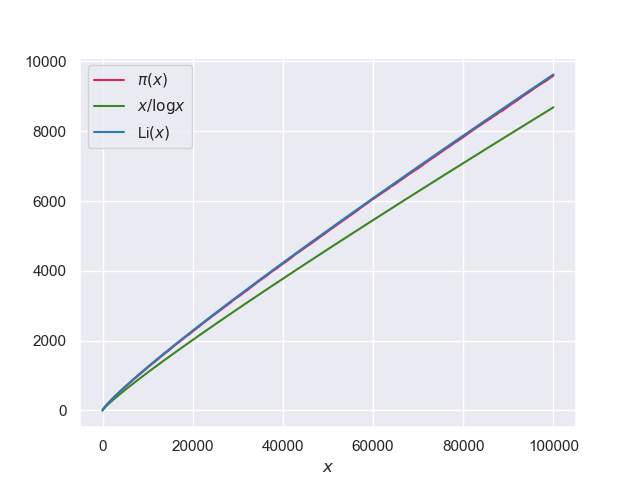
\includegraphics[width=0.8\textwidth]{Chapter1/growth_rates.png}
    \caption[A comparison of the growth of $\pi(x)$, $\textrm{Li}(x)$, and $x/\log x$ for values up to $x = 100,000$. This illustrates plainly how well $\textrm{Li}(x)$ approximates $\pi(x)$.]{A comparison of the growth of $\pi(x)$, $\textrm{Li}(x)$, and $x/\log x$ for values up to $x = 100,000$. This illustrates plainly how well $\textrm{Li}(x)$ approximates $\pi(x)$. \protect\footnotemark}
    \label{fig:my_label}
\end{figure}
\footnotetext{Plot made using Python 3.7.4 with the library Seaborn 0.10.0}